\documentclass{gatech-thesis}
\usepackage{cite}
\usepackage{graphicx}
\usepackage{wrapfig}


%%
%% This example is adapted from ucthesis.tex, a part of the
%% UCTHESIS class package...
%%
\title{Search for Neutrino Transients Using IceCube and DeepCore}
\author{Jacob D. Daughhetee}
\principaladviser{Professor Ignacio Taboada}
\committeechair{Professor Pablo Laguna}
\firstreader{Professor Nepomuk Otte}
\secondreader{Professor Carol Paty\\(Earth and Atmospheric Science)}
\thirdreader{Professor John Wise}
%%\fourthreader{Professor }
\department{School of Physics}
\degree{Doctor of Philosophy}
\copyrightyear{2014}
\submitdate{December 2014}
\bibfiles{example-thesis}
%% The following are the defaults
%%    \titlepagetrue
%%    \signaturepagetrue
%%    \copyrightfalse
%%    \figurespagetrue
%%    \tablespagetrue
%%    \contentspagetrue
%%    \dedicationheadingfalse
\bibpagetrue
%%    \thesisproposalfalse
%%    \strictmarginstrue
\begin{document}
\bibliographystyle{gatech-thesis}
%%
\begin{preliminary}
\begin{dedication}
\null\vfil
{\large
\begin{center}

\end{center}}
\vfil\null
\end{dedication}
\begin{preface}
This dissertation is based on data acquired with the IceCube Neutrino Observatory whose maintenance and operation is the result of an immense international collaborative effort. The bulk of the work pertaining to experimental hardware, data acquisition, reconstruction algorithms, systematics, and simulation presented in this document can be attributed to many IceCube collaborators. However, the refinement of the event selection and subsequent analysis of the data are the original work of the author.
\end{preface}
\begin{acknowledgements}
I want to thank my fellow graduate student office mates whose constant distractions helped me retain my sanity.
\end{acknowledgements}
% print table of contents, figures and tables here.
\contents
% if you need a "List of Symbols or Abbreviations" look into
% gatech-thesis-gloss.sty.

\begin{summary}

% Long Comments
\long\def\/*#1*/{}
\/*
*/

*Observations indicate that there is a correlation between long duration gamma-ray bursts (GRBs) and core-collapse supernovae (SNe).  The leading model for GRB production assumes that relativistic jets are generated by the core-collapse within the progenitor star.  Charged particles undergo Fermi-acceleration within internal shocks of these jets and subsequently give rise to gamma ray emission once the jets breach the surrounding stellar envelope.  Very few SNe result in the occurrence of GRBs, however,  but it has been suggested that a significant fraction of core-collapse SNe manage to produce mildly relativistic jets.  These jets are insufficiently energetic to break through the envelope and are effectively 'choked' resulting in a lack of observed gamma ray emission.  In both the failed and successful GRB scenario, neutrino production can occur if protons are accelerated in the internal shocks of these jets.  These neutrinos may be detectable by the IceCube neutrino observatory and its low energy extension DeepCore. This thesis presents the methods and results of a dedicated search for temporal and spatial clustering of neutrino events during the IceCube 2012 data season.

*Needs tweaking, actual result*


\end{summary}

\end{preliminary}
%%
\chapter{Introduction}
The expansion of traditional optical astronomy into wavelengths unobservable to the human eye revealed myriad phenomena previously unknown to science. Use of wavebands of light spanning several orders of magnitude allowed for the discovery of completely new astronomical sources. Additionally, it allowed for the study of inherently different physical processes within and around source objects. Yet, for all the vast advances in our understanding of the universe the opening up of the electromagnetic spectrum has brought us, it relies entirely upon the physical properties of its messenger particle, the photon.

Absorption of light, either by intervening matter or other background photons, limits the number and type of source objects optical astronomy can hope to observe or characterize. In order to explore regions of high density as well as very high-energy processes, entirely different methods of observation are required. The limitations imposed by light-based astronomy have led to the dedicated investigation of other particles and phenomena as potential cosmic messengers.

\chapter{Neutrino Astronomy}
The nascent field of neutrino astronomy began in earnest with the detection of supernova 1987A, the first extra-solar neutrino point source.
%% Why neutrinos
%% How neutrinos (production, detection)
%% SN1987A
%% GRBs, SN, Chk GRBs

%%
\chapter{Detector}
\subsection{IceCube and IceTop}
The IceCube Neutrino Observatory \cite{2006APh....26..155I} is km$^{3}$-scale neutrino detector located deep within the glacial ice of the Antarctic ice sheet at the geographical South Pole. This location provides IceCube with a pristine detection medium in addition to mechanical support for the entirety of the array. The detector consists of 5,160 light sensors known as digital optical modules (DOMs) which are distributed along 86 cables (referred to as strings) that supply power and provide communication to the surface. Each cable is instrumented with 60 DOMs spaced 17 meters apart starting at 1450 meters below the surface and terminating at 2450 meters below. A inter-string spacing of 125 meters on average results in a total instrumented volume of approximately 1 km$^{3}$. Figure \ref{fig:icecube} provides a schematic illustrating the detector geometry.

\begin{figure}[ht]
  \begin{center}
    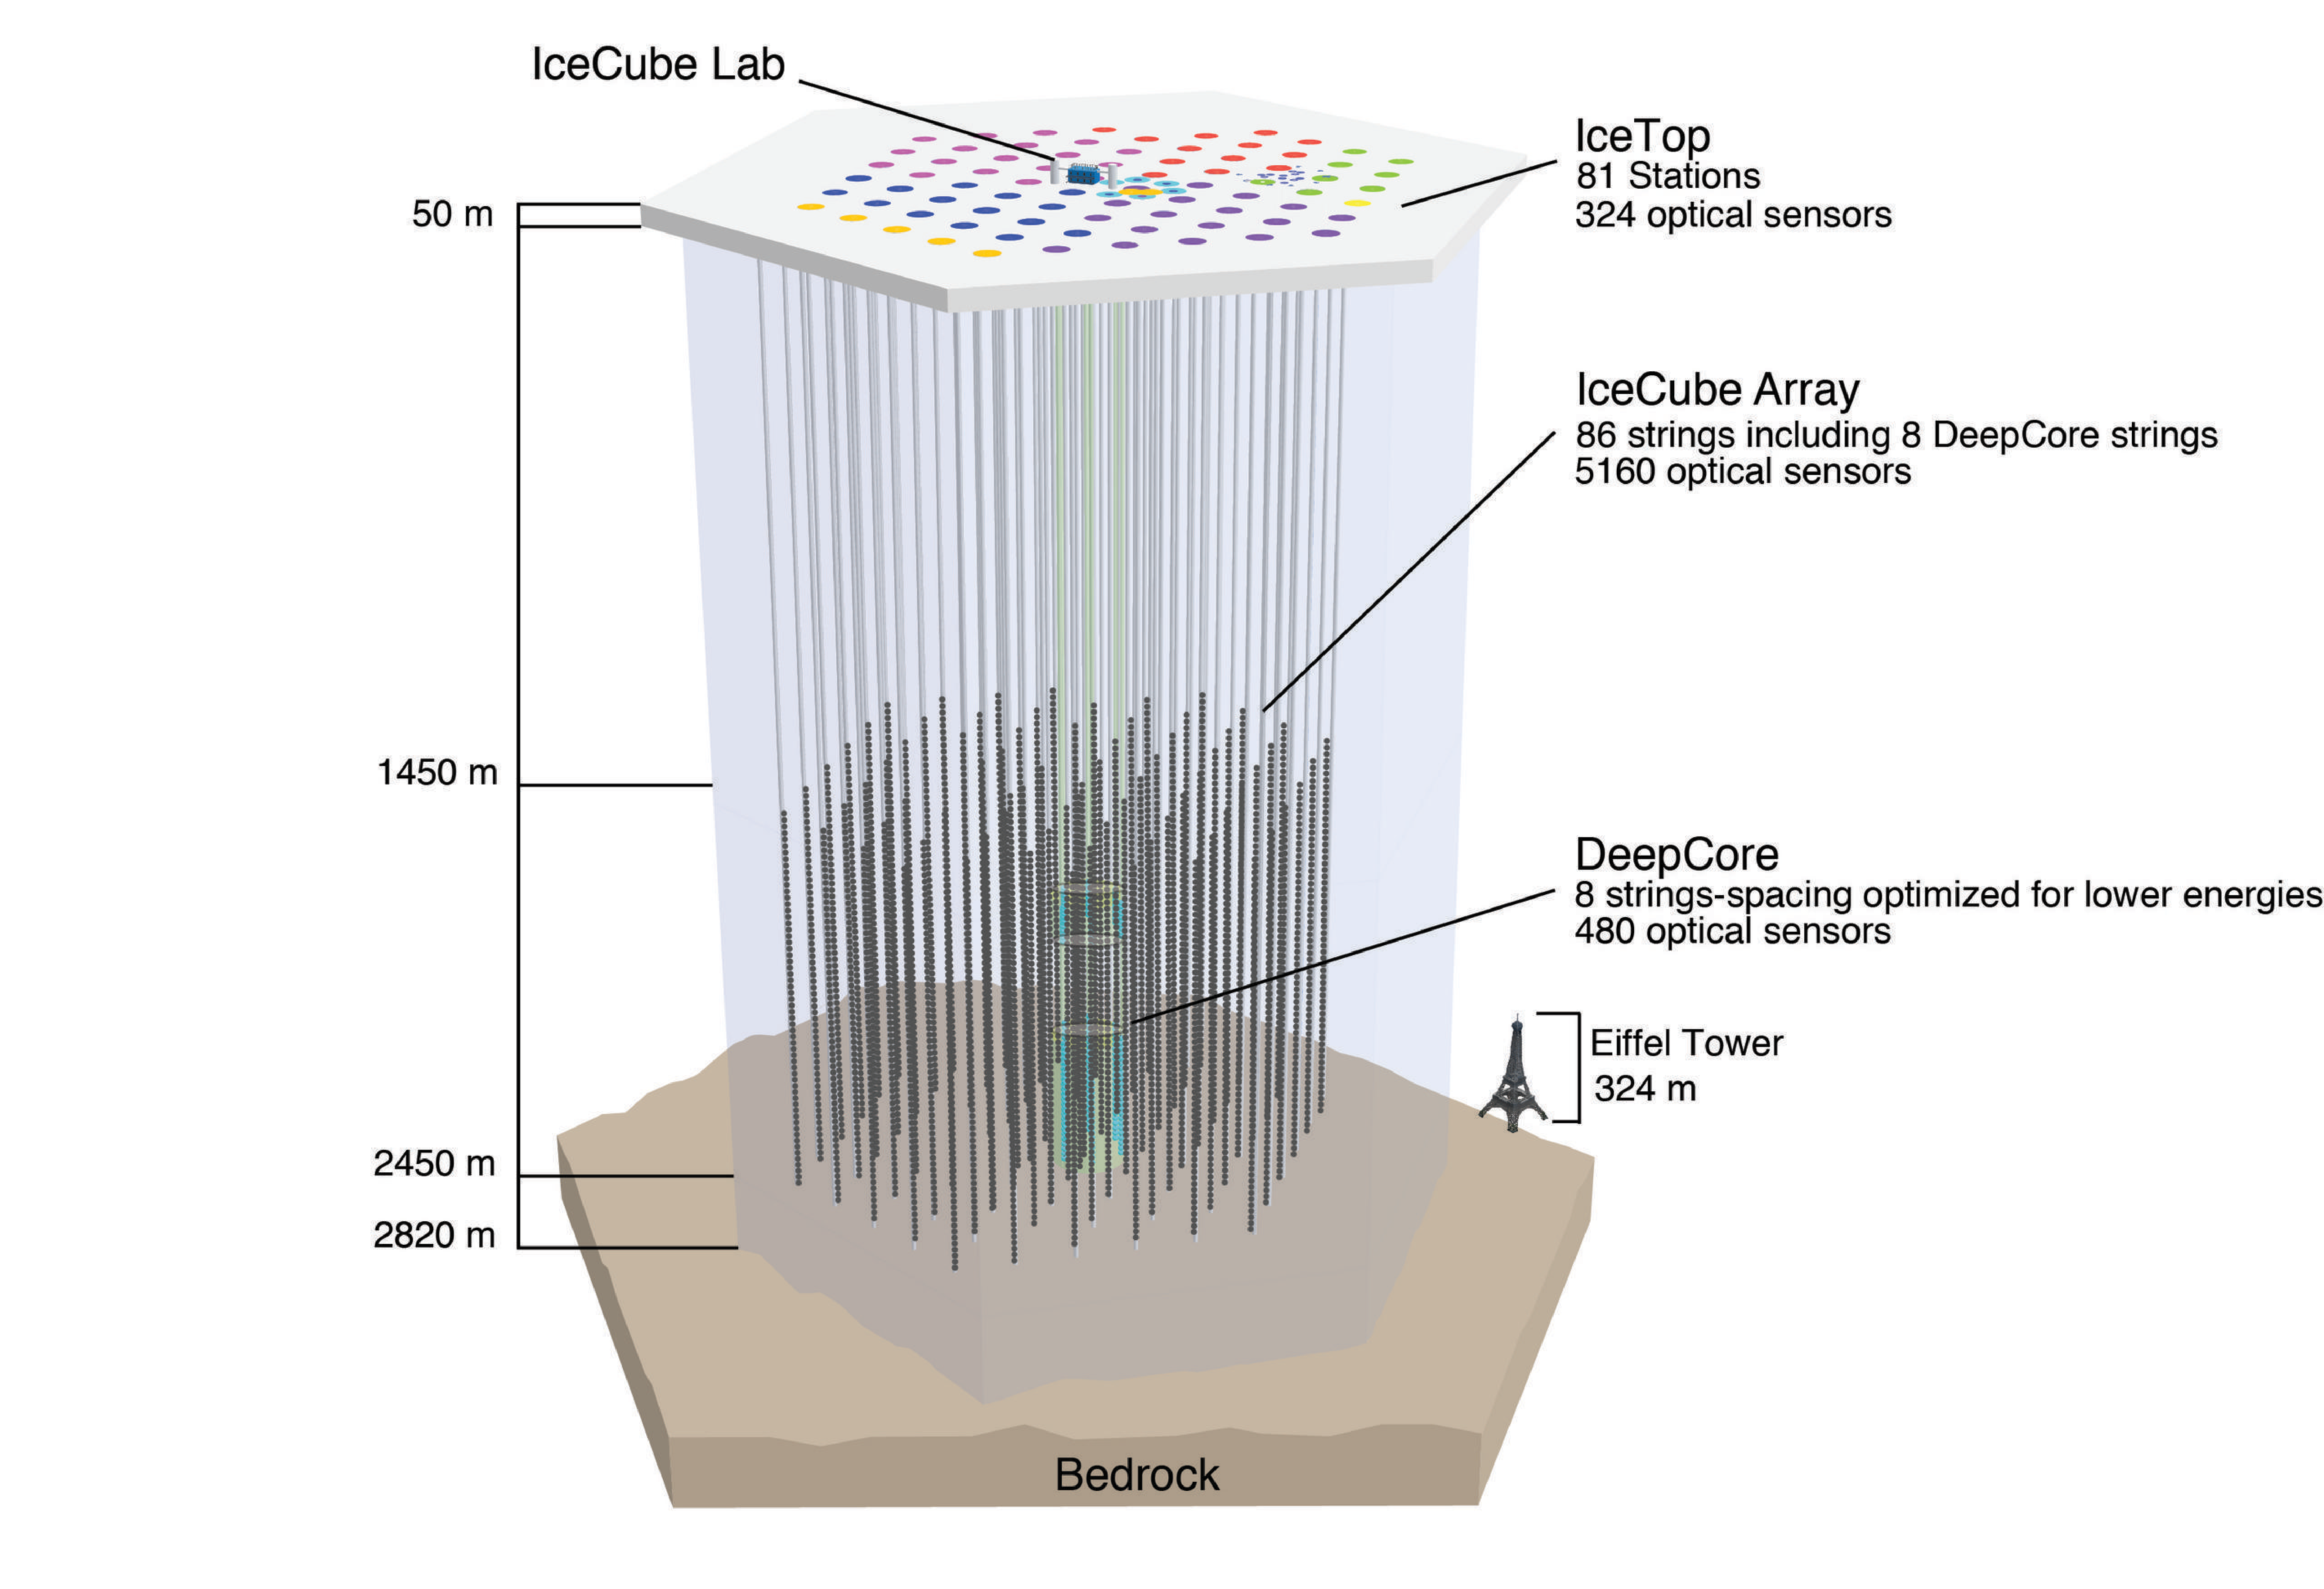
\includegraphics[width=0.83\textwidth,keepaspectratio]{ArrayWSeasonsLabels.pdf}
  \end{center}
  \caption{Diagram of the IceCube Neutrino Observatory (IceCube Collaboration).}
  \label{fig:icecube}
\end{figure}

Installation of the IceCube strings took place over several years and required the use of a specialized hot-water drill. In the deployment process, the hot-water drill is used to bore through the ice leaving a water-filled column in which the string and its attached DOMs are lowered. The water column subsequently freezes the cable and all DOMs in place rendering them completely inaccessible from the surface. The deployment of the first IceCube string occurred on January 29th, 2005. The remaining strings were deployed over the next five summer seasons resulting in data seasons of different detector shapes and size. The final string was deployed on December 18, 2010 giving IceCube its ultimate 80-string configuration.

%%% IceTop

\subsection{DeepCore}

DeepCore \cite{2012APh....35..615A} is a sub-detector deployed in tandem with IceCube between 2009 and 2010 primarily designed to lower the energy threshold of IceCube. The array consists of eight infill strings located in the center of the IceCube detector in addition to the first layer of surrounding standard IceCube strings. This configuration gives DeepCore three layers of IceCube strings to use as an active veto for the primary background of atmospheric muons. In order to improve detector response to lower energy neutrinos, $\mathcal{O}$(10-100 GeV), the infill strings of DeepCore have a much closer inter-string separation (~42 m) and have 50 DOMs spaced 7 m apart deployed deep in the ice between 2100 m and 2450 m. This denser instrumentation allows for better timing and spatial resolution of charged secondaries produced in neutrino interactions.

The depth selected for deployment of the DeepCore DOMs was determined via examination of the ice properties previously mapped by both the Anatarctic Muon and Neutrino Detector Array (AMANDA) \cite{2006JGRD..11113203A} and pre-existing IceCube configurations \cite{2013JGlac..59.1117.}. These investigations into the optical properties of the ice revealed that the deepest ice (< 2100 m) had superior optical qualities with respect to the ice closer to the surface. Additionally, it was determined that a layer of high dust concentration in which light is scattered and absorbed to a much higher degree exists at a depth of 2000-2100 m.

%% Refs: Performance of DeepCore, IceCube construction paper?

\subsection{The Digital Optical Module}
The essential component of the IceCube detector is the DOM. Each of these sensor units contains a photo-multiplier tube (PMT), attached digitizing electronics, and LED flashers all housed within a glass pressure vessel \cite{2006NIMPA.567..214H}. A penetrator cable breaches the pressure vessel to connect the DOM electronics to the supporting string cable enabling DOM-to-DOM as well as DOM-to-surface communications.

\begin{figure}[ht]
\centering
\begin{minipage}[b]{0.45\linewidth}
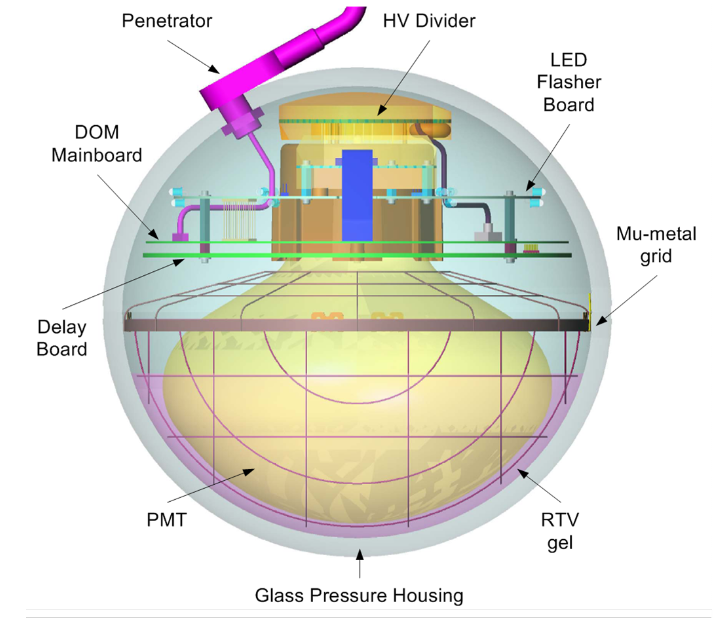
\includegraphics[width=0.95\textwidth]{DomSchematic.png}
\caption{Schematic detailing DOM structure \cite{2009NIMPA.601..294A}.}
\label{fig:domscheme}
\end{minipage}
\quad
\begin{minipage}[b]{0.45\linewidth}
\begin{center}
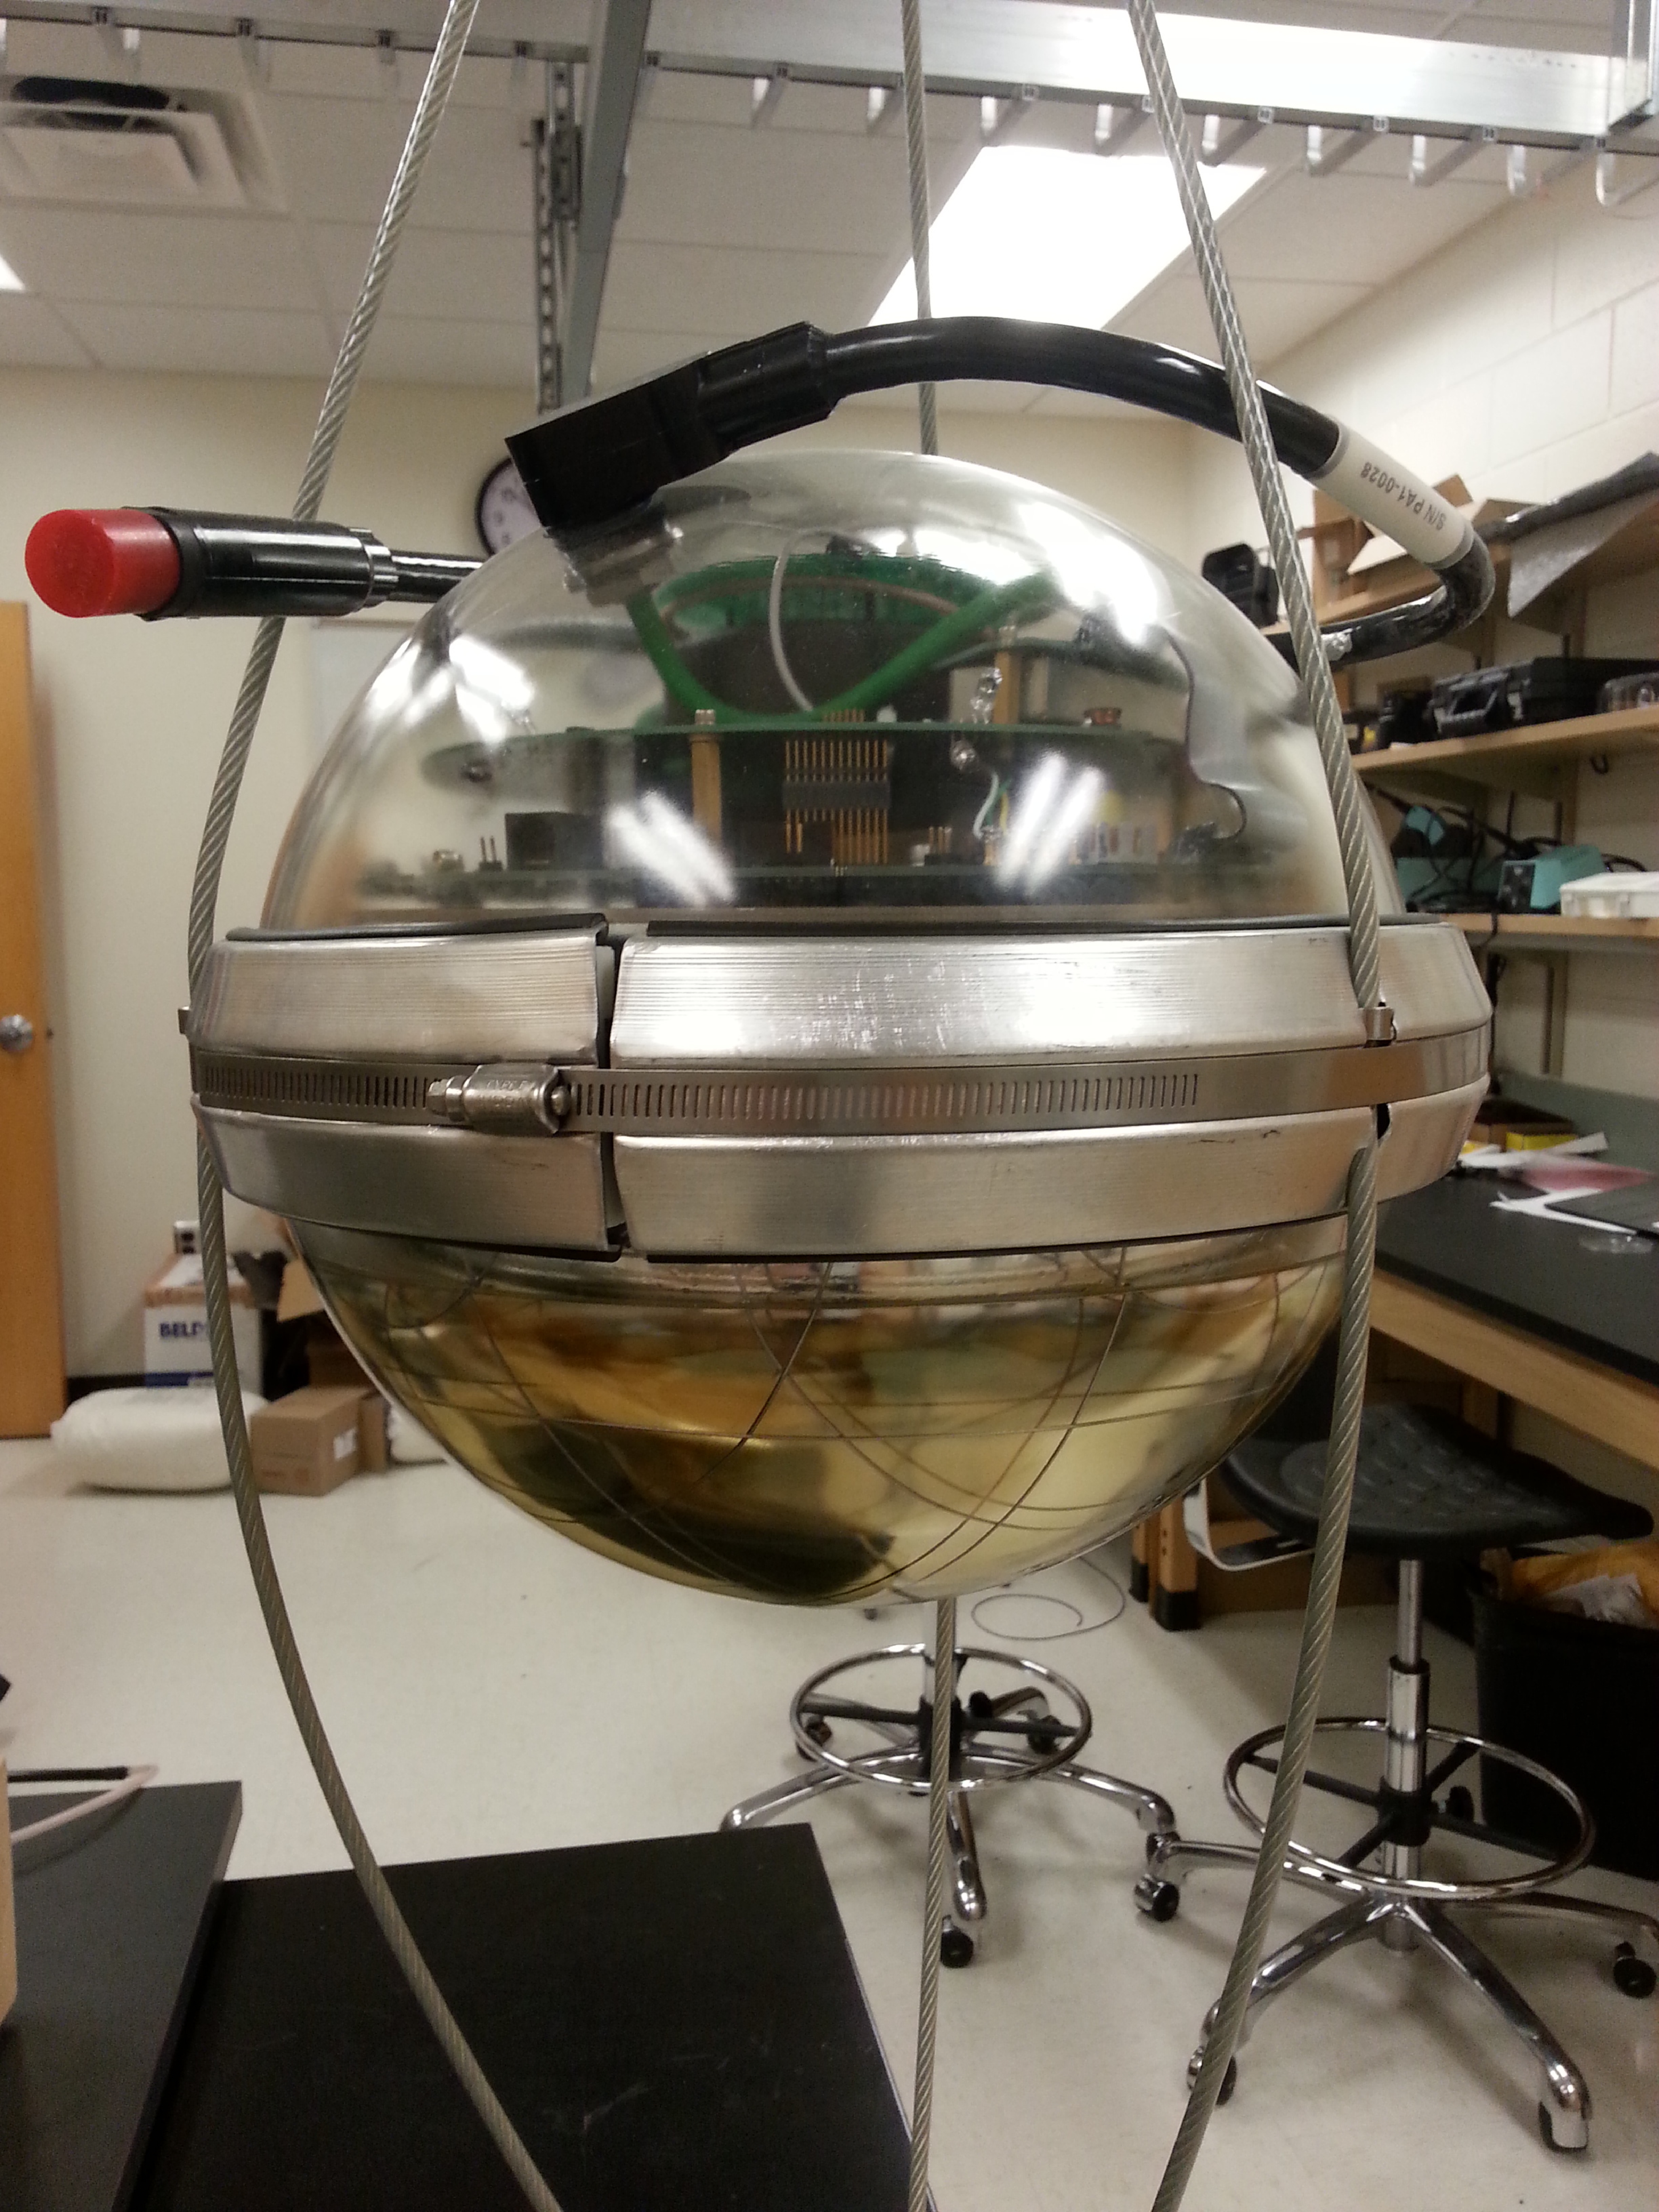
\includegraphics[width=0.75\textwidth]{LabDOM.pdf}
\end{center}
\caption{A fully assembled DOM supported by a cable harness.}
\label{fig:dompic}
\end{minipage}
\end{figure}

\chapter{Data Acquisition}

All data acquisition begins with the registering and processing of photon hits in individual DOMs.


\chapter{Event Selection}

\chapter{Analysis Method}

\chapter{Systematics}
There are many systematic uncertainties that can affect the interpretation of the results of this analysis. The primary contributors to uncertainty being the /it{in situ} scattering and absorption properties of the ice medium and the absolute quantum efficiency of the PMTs within the DOMs.
\chapter{Results}

\chapter{Interpretation}



%%
\chapter{Conclusion}

%% We need this since this file doesn't ACTUALLY \cite anything...
%%

\appendix
\chapter{Appendix Placeholder}

Ancillary material should be put in appendices, which 
appear just before the bibliography. 

\begin{postliminary}
\bibliography{jdthesis}{}

\postfacesection{Index}{%
%%             ... generate an index here
%%         look into gatech-thesis-index.sty
}
\begin{vita}

\end{vita}
\end{postliminary}
\end{document}
